\section{Problem 4}
\label{part4}
\subsection*{Question}
\begingroup
\begin{verbatim}
Use MDS to create a JPEG of the blogs similar to slide 29.  
How many iterations were required?
\end{verbatim}
\subsection{Answer}
\begin{enumerate}
\item The blog space is generated using multidimensional scaling from the script \verb+makeMDS.py+ shown in Listing \ref{lst:mds-code}, which makes use of Toby Segaran's \emph{clusters.py} using the functions \emph{scaledown} on line $7$ and \emph{draw2d} on line $9$.


\lstinputlisting[language=python, frame=single,breaklines=true, caption={Python script for generating a MDS from the blog data},captionpos=b, numbers=left, showspaces=false,label=lst:mds-code, showstringspaces=false, basicstyle=\footnotesize]{questions/q4/makeMDS.py}

\item unfortunately the blog space produced does not fit well on a letter-sized page shown in Figure \ref{fig:q4MDS}.
\item Listing \ref{lst:q4output} shows the output from running this script, which took $253$ iterations on this run.
\end{enumerate}
\newpage
\begin{figure}[h]
\centerline{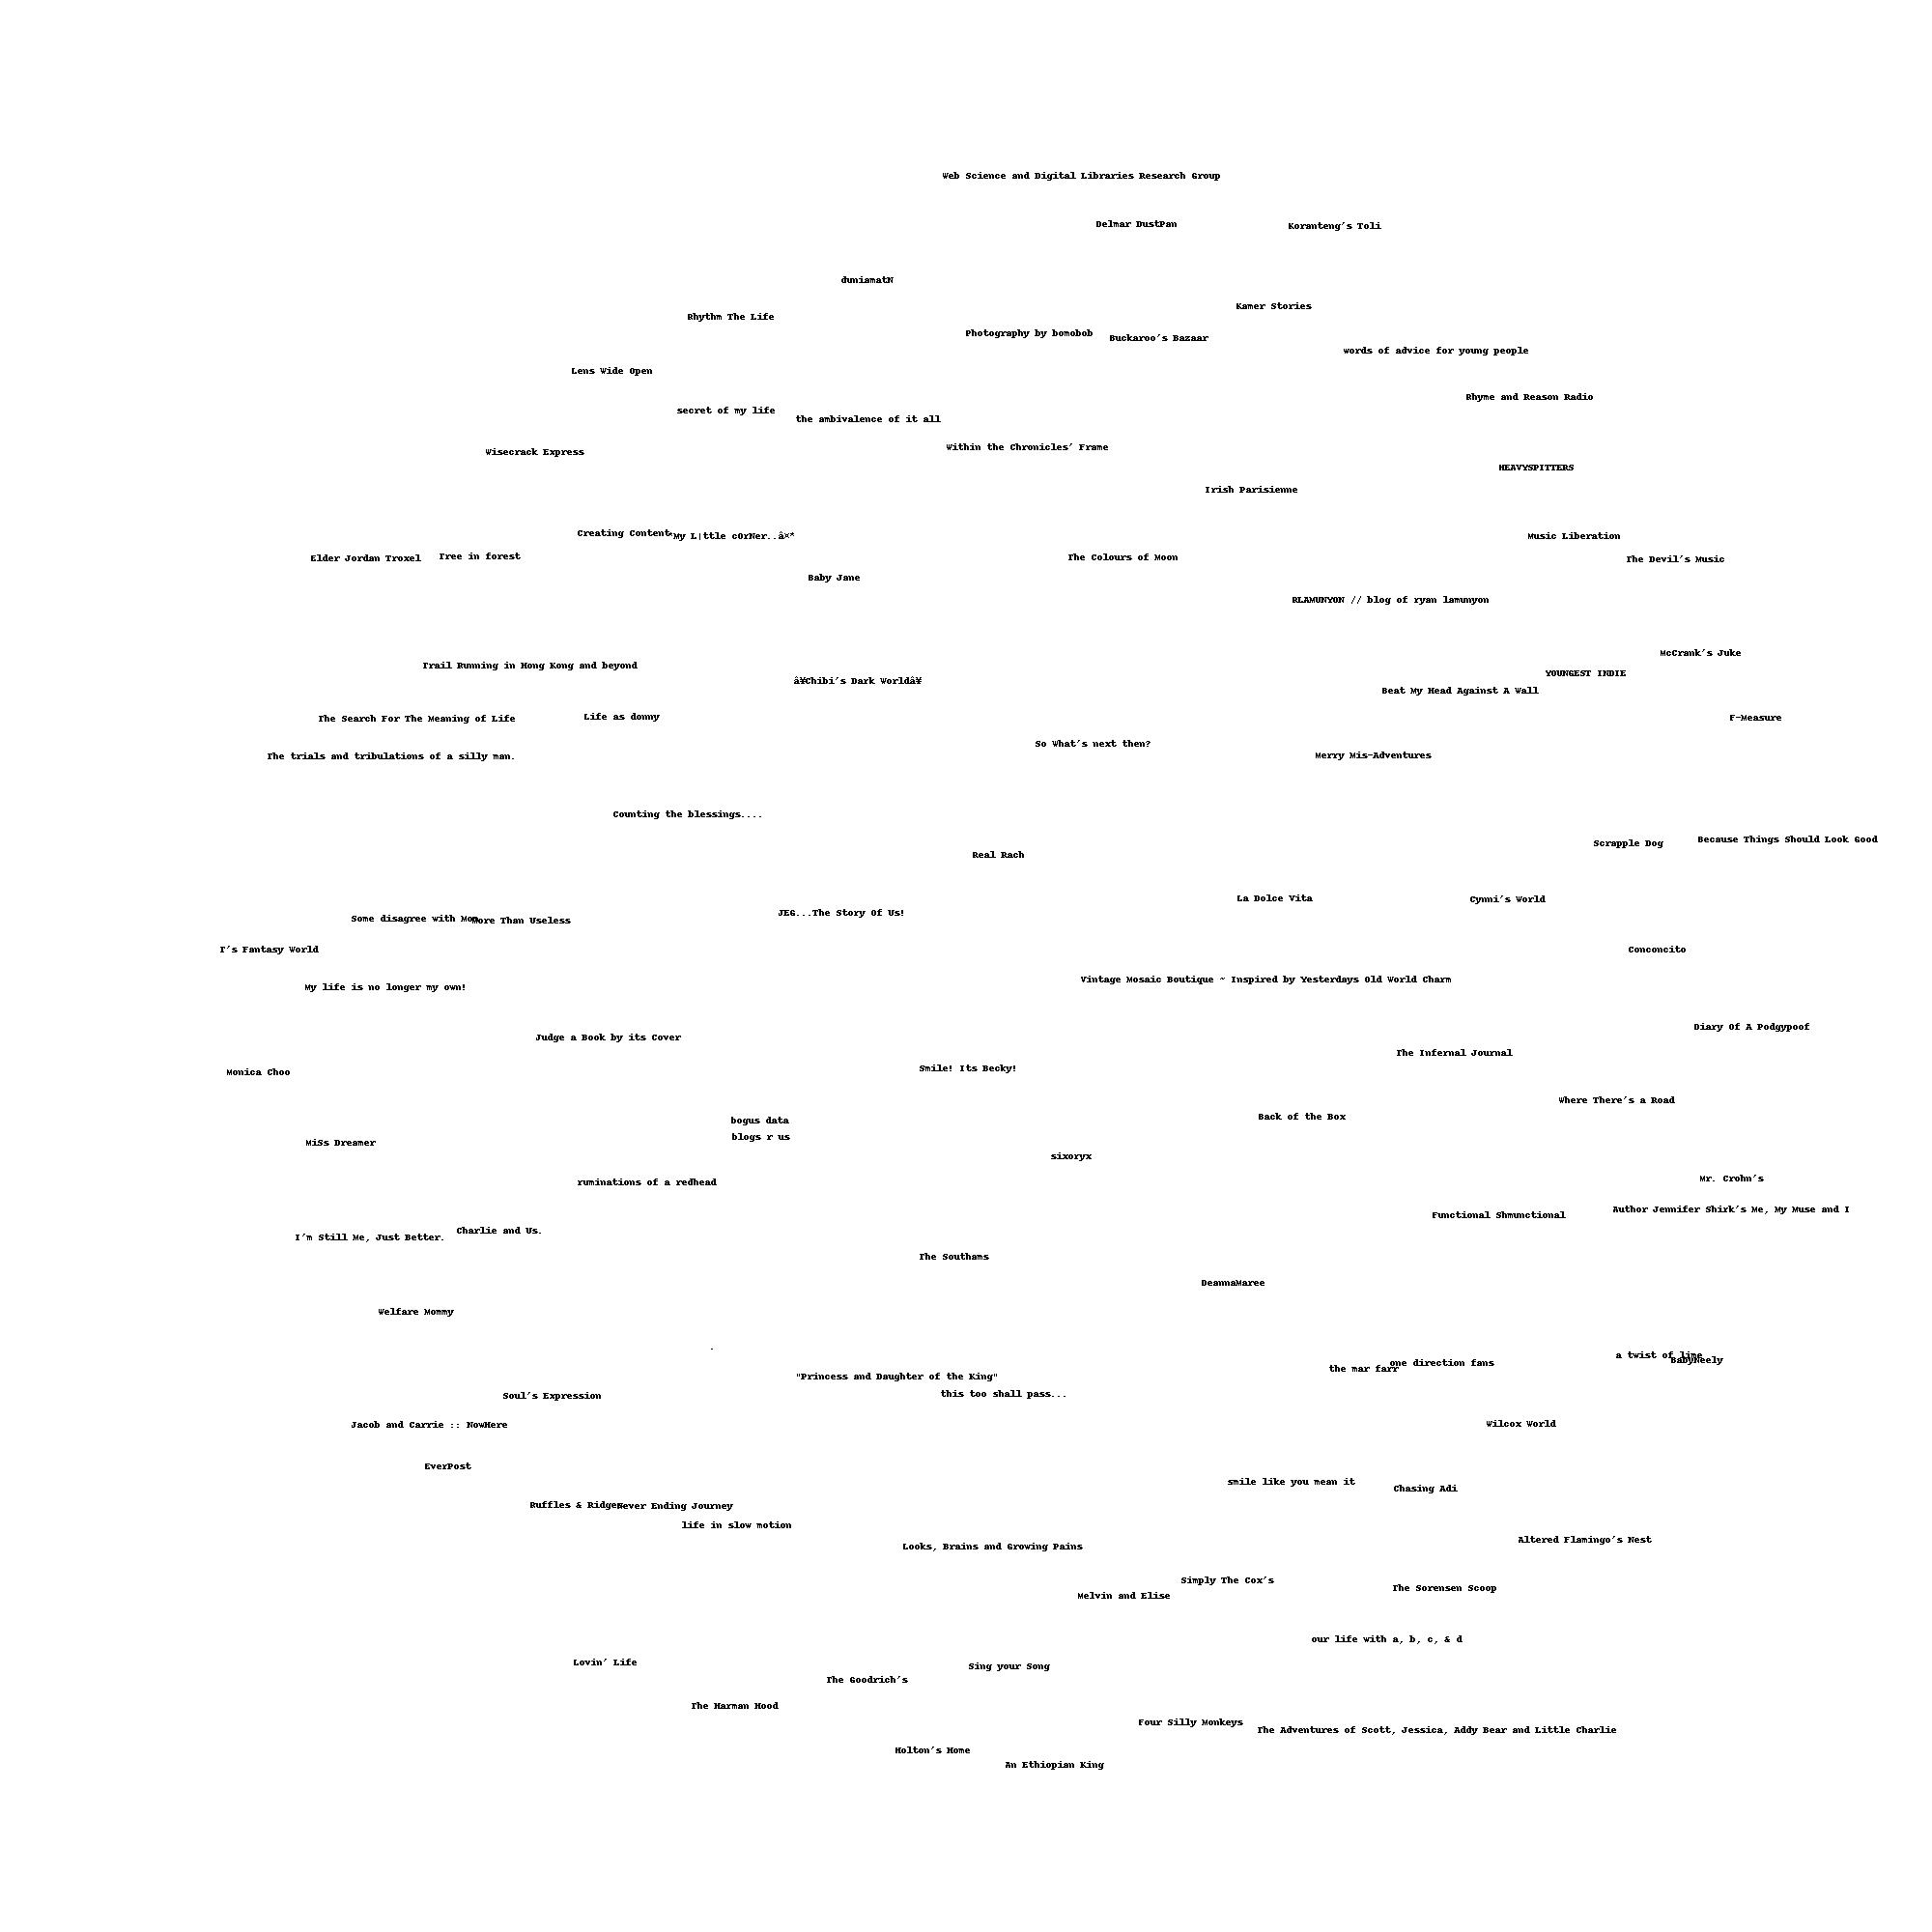
\includegraphics[scale=0.26]{questions/q4/blogs2d.jpg}}
\caption{Blog space produced by the \emph{makeMDS.py} script}
\label{fig:q4MDS}
\end{figure}

\lstinputlisting[frame=single,caption={Output from script \emph{makeMDS.py}},label=lst:q4output,captionpos=b,numbers=left,showspaces=false,showstringspaces=false,basicstyle=\footnotesize]{questions/q4/q5-mds.txt}
\newpage
